\chapter{Methods for inferring pairwise co-location}

With the data extracted and formatted in suitable manner, as described in the previous chapter, we move on to the main part of the thesis. Given a set of consecutive Bluetooth RSSI measurements, \textit{can we infer co-location?}; and if yes, what is the best way of doing it? 

One way of answering these questions is to simply set a threshold, and split the dataset into two parts: the ones that are above the threshold indicate co-location, while the other do not. That is exactly what \textit{Sekara,Lehmann} did in \cite{vedran}, with convincing results. They set the threshold to \textit{ -80 dBm}. 

On a similar note, we average our two types of data, the ones tagged \textit{yes} and \textit{no}, and we obtain an average of \textit{-64 dBm} for the ones tagged \textit{yes} and an average of {-82 dBm} for the ones tagged \textit{no}. From this result, one can easily see the similarity between the threshold in \textit{Sekara,Lehmann}'s work and the values obtained through this thesis's data. 

The above method can successfully be used under any type of measurements. However, it does not take advantage of the additional information that our method of data gathering has provided, such as temporal information, or the significance of continuous measurements. Below we propose three methods of inferring pairwise co-location in the form of three machine learning algorithms. For each one we will provide a theoretical overview and implementation details, followed by a discussion of the results. The chapter will end with a comparison between the three algorithms where results, ease of use and performance will be taken into consideration.

In Section~\ref{sec:data_merger} we split our data into time windows. At any one point during the execution of the algorithms, we will be referring to a single time window, the one for which we want to infer co-location. Of course, additional parameters and features will be used, but even if not specified, every run of any algorithm described below will include, even if not specifically noted, at least the RSSI of a single time window, the one mentioned at the beginning of this paragraph. 
 
While the parameters and the inputs used differ from one algorithm to another, one thing that remains constant across all of them is the testing methodology, described in the following section.

\section{Testing methodology}

In order to test the accuracy of the algorithms, we use cross-validation, a well recognized method for computing accuracy estimations \cite{kohavi1995study}. The technique is used here for obtaining an accuracy score for each algorithm and its variations, so that a comparison can be made at the end. Broadly speaking, cross-validation refers to the techniques used to partition the main dataset into two sets: a \textit{training} set, used in the initial phase for training the algorithms, and a \textit{testing} set, used for validating the algorithm with \textit{unseen before} data, after the training has finished. Two methods were used: k-fold validation, with $k = 10$ \cite{kohavi1995study}, and repeated random sub-sampling validation, with a $80-20$ proportion \cite{segaran}. 

\begin{itemize}
  \item K-fold validation is done by partitioning the data in k sets. One set is used for testing, while the the other $k-1$ are used for training. The processed is repeated $k$ times, once for each partition. The end result is the average over all $k$ results obtained. 
  \item For random sub-sampling validation, the dataset is partitioned into two sets. The entries are randomly assigned to one of the sets based on the proportion established at the beginning. For this type of validation, the test has been repeated 100 times, and the results averaged.   
\end{itemize}

During the execution of the tests, both k-fold validation and repeated random sub-sampling validation output extremely similar results, most of the time the results having less than $0.5\%$ difference between them. For this reason, when presenting an algorithm score, that score will be the average of the two methods. 


\section{Neural Networks}

A first approach aims to use artificial neural networks (ANN) in order to infer co-location. Specifically, this section will deal with feed-forward ANNs, both from a theoretical and a practical point of view. 

\subsection{Theoretical overview}

The introduction of backpropagation by Rumelhart et al. \cite{rumelhart} paved the way for the development of the modern artificial neural network. In their current form, ANNs can be described as a set of processing units, called \textit{neurons}, or \textit{artificial neurons} that communicate between each other. 

The general layout of a feed-forward ANN can be seen in Fig. \ref{pic:ann}. It consists of an input layer, one or more hidden layers and an output layer. The number of \textit{neurons} on the input layer is equal with the number of features that represent the object we need to classify. The number of \textit{neurons} in the output layer usually equals the number of classes the objects need to be classified in. The number of hidden layers, and the number of \textit{neurons} in those layers varies greatly from problem to problem, and will be discussed in the next section, which tackles the implementation details.
In addition to the processing units, the other major components of a feed-forward network are the links between the \textit{neurons}. They type of ANN described here is feed-forward, which means the links are uni-directional. Information only moves from the input \textit{neurons}, to the \textit{neurons} in the hidden layers, to the \textit{neurons} in the output layers. For example, in Fig. \ref{pic:ann}, information only moves from left to right \cite{annintroduction2}.  

\begin{figure}[h]
	\begin{center}
		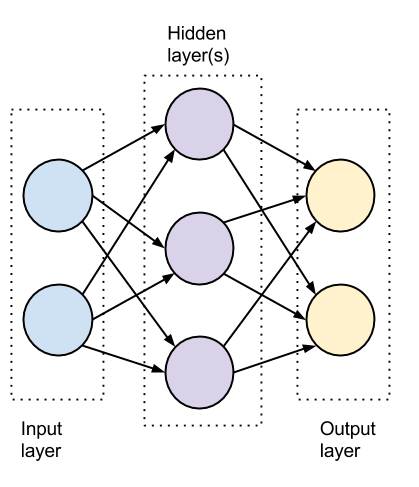
\includegraphics[scale=0.6]{figures/ANN.png}
	\end{center}
	
	\caption{General structure of an ANN.}
	\label{pic:ann}

\end{figure} 

An artificial neural network gets its name from the similarity it has with the biological network of neurons one finds in the human or animal brain. The same can be said about the way it works. Each \textit{artificial neuron} receives an input from all the other \textit{neurons} on the previous layer (or they receive outside input if they are on the input layer). Once all the inputs are received, the \textit{neuron} in question processes them and outputs the result to \textit{neurons} on the next layer \cite{annintroduction}. Fig. \ref{pic:neuron} shows the details of an \textit{artificial neuron}.

\begin{figure}[h]
	\begin{center}
		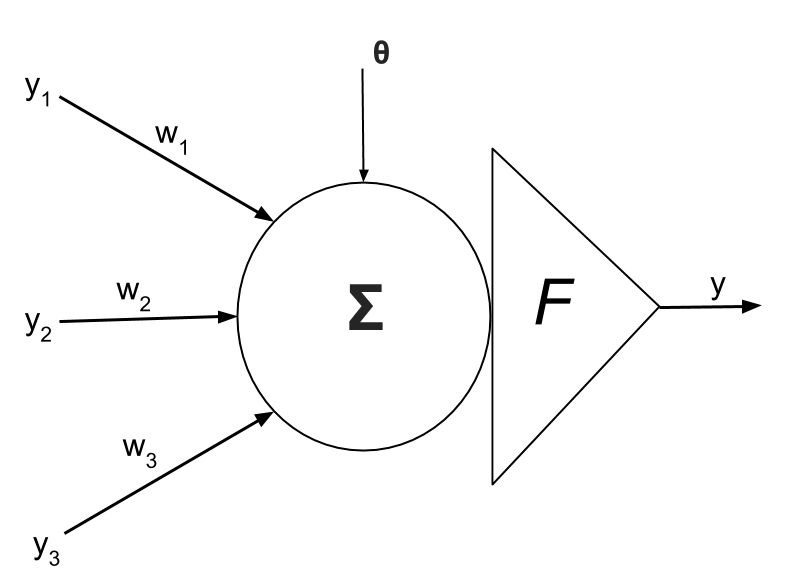
\includegraphics[scale=0.3]{figures/neuron.png}
	\end{center}
	
	\caption{Structure of an artificial neuron.}
	\label{pic:neuron}

\end{figure}

Each link between \textit{neurons} is characterized by a weight, $w_i$. A \textit{neuron} applies a so-called \textit{activation function} on the weighted sum of the inputs, and outputs the result. Sometimes, a bias is used: $\theta$. Thus, the output of single \textit{neuron} can be expressed as:

\begin{equation*}
y = F(\sum_i w_i y_i + \theta)
\end{equation*}

\begin{description}
  \item[$y$]   The output of the current \textit{neuron}.
  \item[$F$]   The activation function. This is usually either the \textit{sigmoid} function, $y = F(x) = \frac{1}{1 + e^{-x}}$, or the \textit{tanh} function \cite{annintroduction}.
  \item[$w_i$] The weight of an input link.
  \item[$y_i$] The input, either from a previous layer of \textit{neurons}, or a from outside the network.
  \item[$\theta$] Bias
\end{description}

In order for the network to output the expected result when presented with an input, it has to be set up. That translates into assigning appropriate values to the weights corresponding to the links between \textit{neurons}. One way of doing this is to manually assign the values. However, this implies a priori knowledge, which is not possible in most cases. The other choice is to \textit{train} the network. 

The training method used here is backpropagation, first introduced in \cite{rumelhart}. The intuition behind is as follows. We randomly assign values to the weights $w_i$ in the ANN. We apply an input to the network, whose result we already know, and compare the outputted result with the correct one. The aim is to minimize the difference. 

While the mathematical procedure through which researchers have reached backpropagation is outside the scope of this thesis, based on \cite{annintroduction} we will present the general equations used in the implementation of the algorithm:

We modify each weight with:  
\begin{equation*}
\Delta w_k = \alpha \delta_k y_k
\end{equation*}

Where $\alpha$ is the learning rate, $y_k$ is the input value on link $k$, and $\delta_k$ is computed as follows:
\begin{equation*}
\delta_k = F'( \sum_i w_i y_i + \theta ) \sum \delta_l w_{kl}
\end{equation*}

Where $\delta_l$ is used in the next layer, and $w_{kl}$ represents a weight between the current layer and the next one. This process continues recursively, until we reach the output layer. In order to finish the computations, we need the $\delta_o$ which corresponds to the output layer:  

\begin{equation*}
\delta_o = (d - y) F'(\sum_i w_i y_i + \theta)
\end{equation*}

Where $d$ represents the expected output, and $y$ the desired output. As one can easily see, we begin from the output layer with computing $\delta_o$, and updating the corresponding weights. We then move further one layer, and compute the corresponding $\delta$ values. We continue to go back until we reach the links that connect to the input layer. From this procedure the \textit{back} in \textit{backpropagation} comes from. 

\subsection{Results}

For implementation purposes we used a Python neural network, available at \cite{issam}. The network used has, besides the mandatory input and output layers, a single hidden layer (which is enough \cite{Hornik1989359,Hartman,cybenko}). 

The number of \textit{neurons} in the hidden layer differs greatly from problem to problem, with some authors suggesting any number between the number of \textit{neurons} in the input layer, to up to two times that value \cite{Stathakis}. Due to the relatively small number of features extracted from the phone data, we have run tests varying numbers of hidden units in the above mentioned range. 

During the testing, different values for the $\alpha$ parameter have been tried, in the end, the values that yielded the best results being between 0.15 and 0.4, with little variation. As such, all the tests that are done below are done with an $\alpha$ parameter of 0.2. 

We begin our testing with the most basic case. We use a single feature, the measured Bluetooth RSSI. The plot in Fig.~\ref{pic:ann_single} details the results obtained. While the accuracy is acceptable, we can easily see that varying the number of hidden nodes in the hidden layer has no impact on the result. 

\begin{figure}[h]
	\begin{center}
		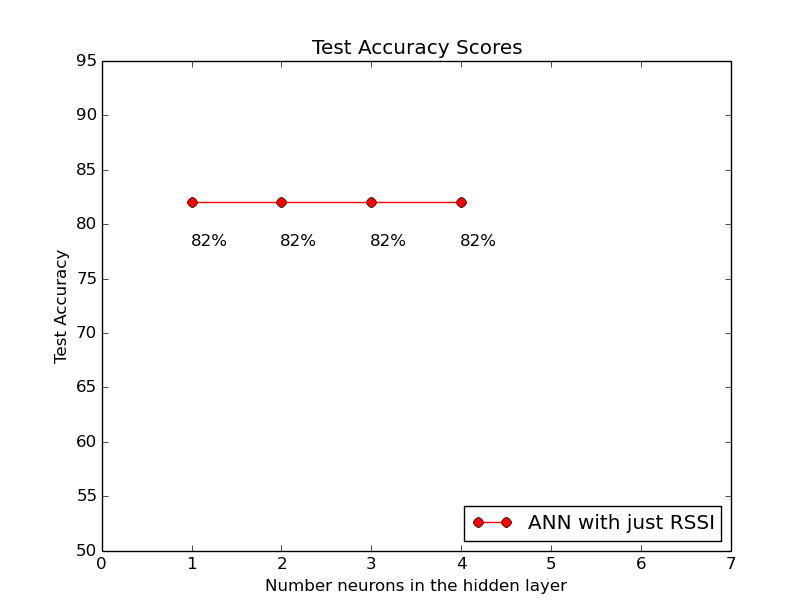
\includegraphics[scale=0.6]{figures/ann_simple.png}
	\end{center}
	
	\caption{Test accuracy for ANN when just the RSSI is used as a feature.}
	\label{pic:ann_single}

\end{figure}

Next we try to make use of the notion of chains, as it was defined in Section~\ref{sec:data_merger}. When trying to infer co-location for a specific time window, we also look at the RSSI of the windows that are in the same chain, but before it. We gradually increased the number of \textit{neurons} in the hidden layer, as well as the number of windows we take into consideration. 

As we increased the number of windows, the length of the chains becomes a problem. Different chains have different lengths, but the number of features in the ANN remains constant. For example, when using four previous windows, and a chain has only a length of three, even in the best case scenario, we still have two missing features. 

One way to deal with this problem is to simply discard the cases that are missing values. However, this introduces significant bias into the data, as observation of the dataset has shown that shorter chains are more likely to belong to the category tagged with \textit{no}. By discarding them, we greatly reduce the number of samples tagged with \textit{no}, thus unbalancing the overall proportion of training and testing data. As such, we used imputation to replace the missing values. Two approaches were used.

A first approach used mean imputation. We replaced the missing data with the average of the values in the chain. Fig.~\ref{pic:ann_params2} shows the results obtained. Secondly, we used last observation carry forward \cite{locf}, as it involved items ordered by time value. The results can be seen in Fig.~\ref{pic:ann_params1}. Consideration has been given to multiple imputation \cite{rubin2009multiple}, however, its cost, and the next result made it unsuitable.  

\begin{figure}[h]
	\begin{center}
		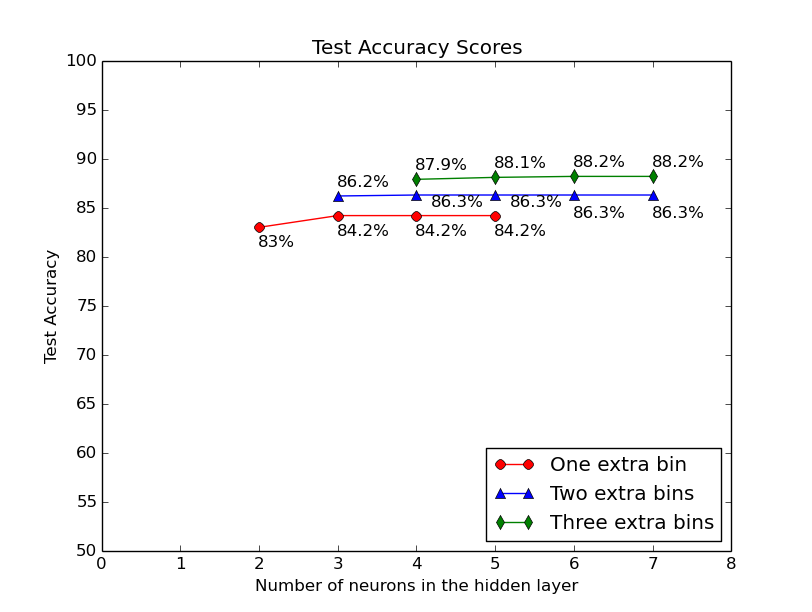
\includegraphics[scale=0.6]{figures/ann_params2.png}
	\end{center}
	
	\caption{Test accuracy for ANN when the RSSI for the current and previous time windows are used as features, with mean imputation.}
	\label{pic:ann_params1}

\end{figure}

As we increase the number of time windows, for mean imputation, the accuracy increases. However, this is due to the uniformization of data, as every value that is missing is replaced with the average. As the average is almost the same between the testing set and the learning set, we end up with entries who sometimes look extremely alike. When entries are full of averages, the difference is made by the real data. As the number of time windows with real data decreases, this choice of parameters comes closer and closer to the basic one. However, even with one extra bin, this choice of parameters is an improvement over it, as every extra time windows has the chance of providing new data.   

\begin{figure}[h]
	\begin{center}
		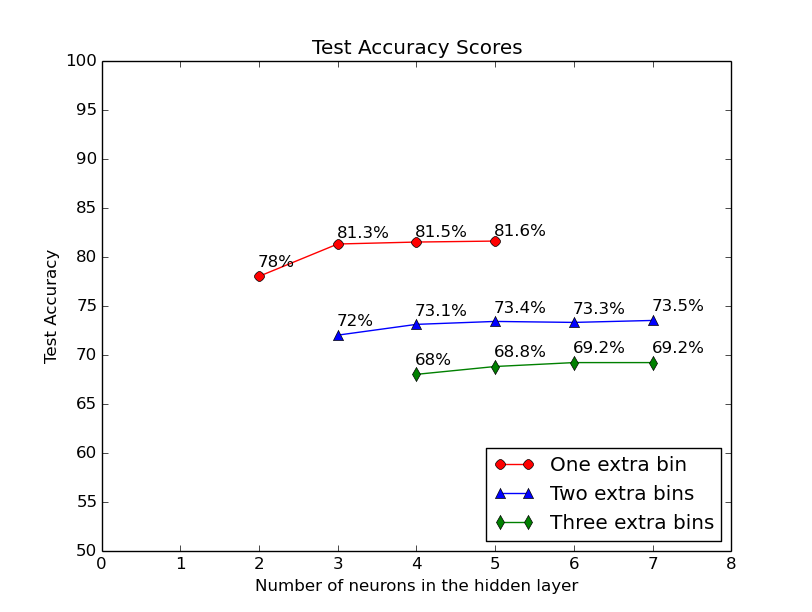
\includegraphics[scale=0.6]{figures/ann_params1.png}
	\end{center}
	
	\caption{Test accuracy for ANN when the RSSI for the current and previous time windows are used as features, with last observation carry forward imputation.}
	\label{pic:ann_params2}

\end{figure}

Running the algorithm with a last observation carry forward strategy for replacing missing values produces negative results. Even taking into consideration the best result of this set, obtained with only one extra time window, we are still below or close to the score of the basic set.  As we increase the number of time windows used, the accuracy drops markedly, with an almost 7\% jump downwards between one and two extra time windows, and a 4\% drop between two and three extra time windows. This choice of parameters is unsuitable for this algorithm.    

Taking into account the additional information provided by the chain that a window belongs to can improve the result. However, the previous approach had a number of issues, related to missing values, and the choice of how many extra time bins should be taken into consideration. For the next set of parameters, we only use two features: the RSSI of the current window, and the length of the chain the window is a part of. This has the strength of avoiding any bias introduced by imputation, while at the same time making almost full use of the additional information provided by the chain. Fig.~\ref{pic:ann_chain} shows the test accuracy for this choice of features.

\begin{figure}[h]
	\begin{center}
		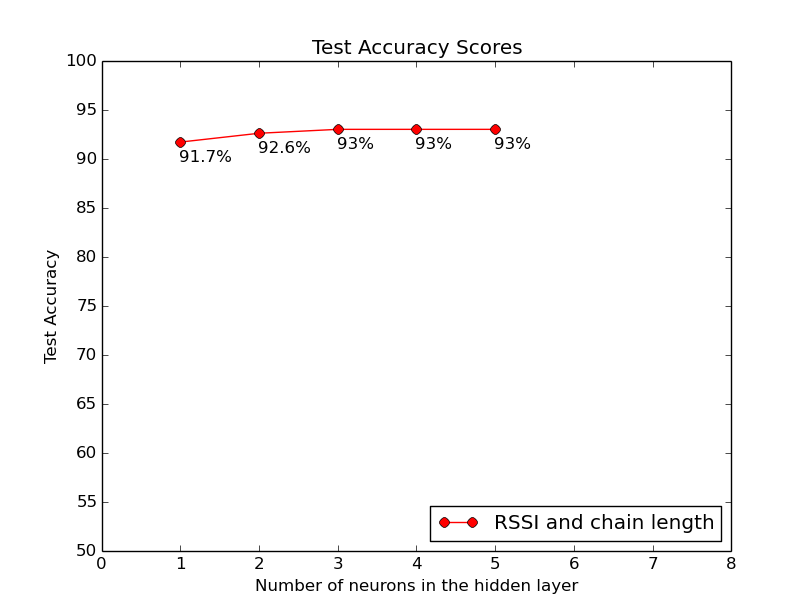
\includegraphics[scale=0.5]{figures/ann_chain.png}
	\end{center}
	
	\caption{Test accuracy for ANN when the RSSI and the chain length are used as features.}
	\label{pic:ann_chain}

\end{figure}

Finally, Fig.~\ref{pic:ann_total} shows a plot with a comparison between the best results for each choice of parameters. Clearly, using just the current window RSSI and the chain length is the best choice. While providing just a minor increase in computation cost by adding just one extra new feature, it is better than the basic case by more than 10\%. The parameter set using mean imputation comes close, but still produces inferior results. Furthermore, the use of imputation raises questions regarding the validity of the obtained result, as well as over-fitting. 

Across the entire suite of tests, the variation in the number of \textit{neurons} had little to no impact on the overall accuracy of the tests. Even with a minimum number of \textit{neurons}, the results were extremely close to cases where four or five were used. The extra \textit{neurons}, however, did had an impact on the overall performance. The difference between using three \textit{neurons} instead of one translated into a doubling of the training and running time. 

\begin{figure}[h]
	\begin{center}
		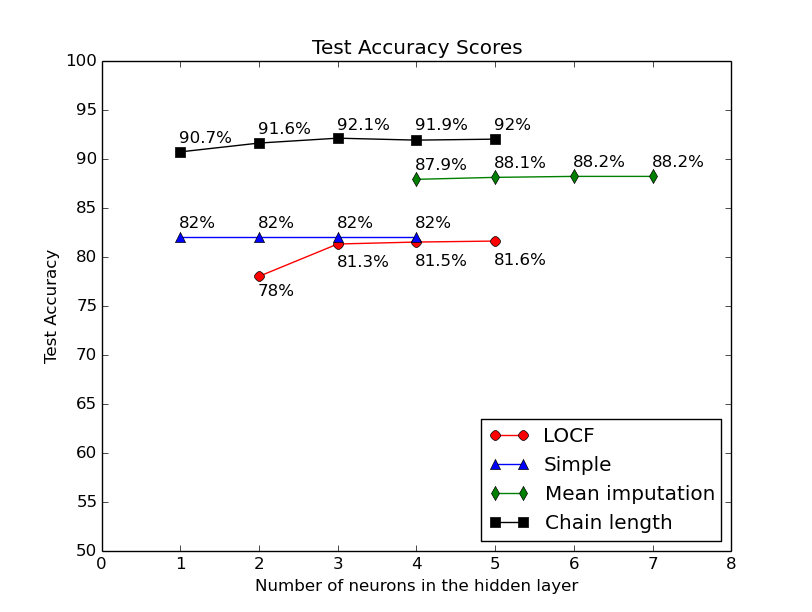
\includegraphics[scale=0.6]{figures/ann_total.png}
	\end{center}
	
	\caption{Comparison between test accuracy for the best cases for each set of parameters.}
	\label{pic:ann_total}

\end{figure}
     

\section{Logistic regression}

In order to meet the objective stated at the beginning of this thesis, we look at the measured Bluetooth RSSI, and some adjacent data, and we try to decide if we have co-location. This can be expressed as the output(response) variable is depending on the input(explanatory) variables  \ref{logmodel}. This immediately leads to the idea of regression. The most basic example of this is the linear regression. However, linear regression has an output variable that is continuous, which is unsuitable for the problem raised by this thesis.

Indeed, here we have a dichotomous outcome. Given a set of measurements, there either is or isn't co-location. For these types of situation, a different type of regression is required, namely logistic regression. 

\subsection{Theoretical overview}

Although usually regressions are used to either predict or estimate a certain value, logistic regression is actually a classifier, thus suitable for our problem. 

The foundation of the logistic regression consists of the logistic function:
\begin{equation*}
f(y) = \frac{1}{1+e^{-y}}
\end{equation*}

Fig.~\ref{pic:logit} shows the plot of the logistic function. It has several attractive qualities. Based on \ref{kleinbaum2010logistic}:

\begin{itemize}
  \item Its output values are between $0$ and $1$. Thus it can easily map probabilities, which is the result of the logistic model.
  \item Looking at Fig.~\ref{pic:logit}, we can discern the presence two points after which the function increases(decreases) significantly , which can be considered activation thresholds, when looking from the point of view of a classifier.  
\end{itemize}

\begin{figure}[h]
	\begin{center}
		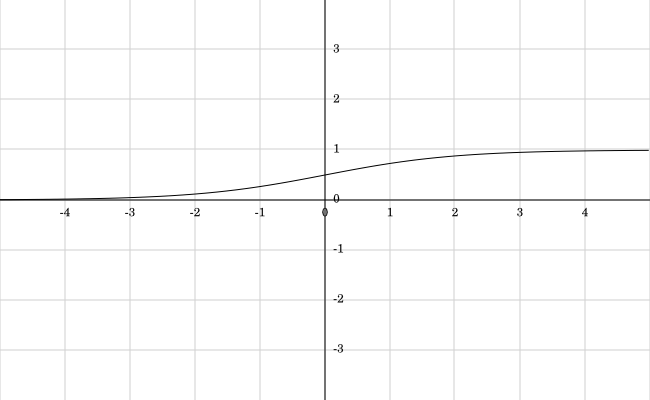
\includegraphics[scale=0.5]{figures/logit.png}
	\end{center}
	
	\caption{Plot of the logisitic function.}
	\label{pic:logit}

\end{figure}

Based on \cite{kleinbaum2010logistic,logmodel,statistics}: for a set of measurements, the logistic model computes the probability that they belong to either one of the categories. We wish to model the dependence between $X$, which consists of a set of variables $X = \lbrace X_1,X_2,X_3,... \rbrace$ and $p(X) = Pr(Y \vert X)$, where $Y$ represents the classifier labels. Using the above logistic function, we can write:
\begin{equation*}
p(X) = \frac{1}{1+e^{-X}}
\end{equation*}

But $X$ can be written as a linear combination of the input variables: $X = \beta_0 + \beta_1X_1 + \beta_2X_2 ...$. Replacing in the above equation we obtain:
\begin{equation*}
p(X) = \frac{1}{1+e^{-(\beta_0 + \beta_1X_1 + \beta_2X_2 ...)}}
\end{equation*}

We also need to compute the \textit{logit}, the inverse of the above function:
\begin{equation*}
ln\frac{p(X)}{1 - p(X)} = \beta_0 + \beta_1X_1 + \beta_2X_2 ...
\end{equation*}

All that is left now is to estimate the unknown quantities $\beta_0, \beta_1, \beta_2...$. This is usually done with maximum likelihood estimation \cite{menard2009logistic}. Intuitively, the method looks for estimates of $\beta_0, \beta_1, \beta_2...$, so that the results obtained using those estimates come very close (or as close as they can) to the expected result. The maximum likelihood estimation makes use of the likelihood function:

\begin{equation*}
l(\beta) = \prod_ip(X_i)[1 - p(X_i)]
\end{equation*} 
Where the first term corresponds to cases that belong to one category, and the second to cases that belong to the other category. The estimations for $\beta_0, \beta_1, \beta_2...$ are chosen so that the above function is maximized. Solving the above equation entails the use of iterative methods \cite{logmodel}, and is outside the scope of this paper.
 
\subsection{Results}

We used the Scikit-learn \cite{scikit-learn} implementation for the logistic regressor. For testing purposes we used the same sets of parameters as before. The results can be seen in Fig. \ref{pic:logic_tot}.

\begin{figure}[h]
	\begin{center}
		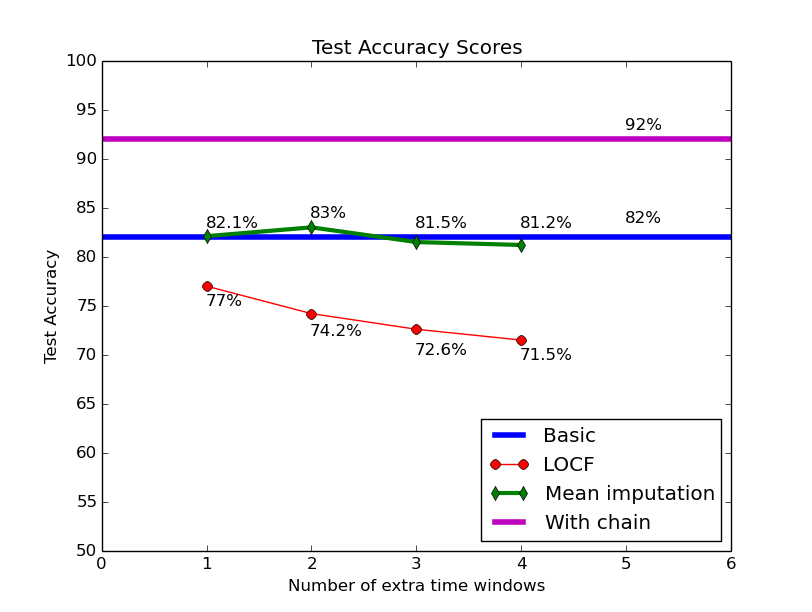
\includegraphics[scale=0.7]{figures/logic_tot.png}
	\end{center}
	
	\caption{Testing results for logistic regression.}
	\label{pic:logic_tot}

\end{figure}

For the basic case, where only the Bluetooth RSSI measurement is used, the accuracy reaches 82\%. We then continue the tests with the use of multiple time windows. Again, in case of missing windows, we use imputation, both mean imputation and last observation carry forward. 

Increasing the number of time windows used has little effect on the mean imputation parameter set, it peaking at 83\%, when two extra time windows were used. This value comes very close to the score obtained with basic set, and also introduces a high amount of computational overhead, from the algorithm (as we add more features, more values need to be estimated), as well as the database structure(as the chain structures need to be traversed). Overall, this choice of parameters brings little against the basic set.

The same cannot be said by the variation that uses last observation carry forward. Increasing the number of time windows taken into consideration has a significant effect on the overall accuracy of the algorithm. Unfortunately, it is not a positive one. As we increase that number, the accuracy decreases dramatically. Even with one extra time window, the score we obtain is lower than even the basic case. When we move to two extra windows, the score drops to 74.2\%, to 72.6\% for three windows, and 71.5\% for four windows, and the trend continues. Clearly, this choice of parameters is not suitable for this particular algorithm. 

The last choice of parameters is the Bluetooth RSSI of the current time window and the length of the chain it belongs to. This set of parameters provides a significant improvement over all the other cases, with an accuracy of almost 92\%. In addition to the improved test score, this choice requires only one new feature to be added to the algorithm, in comparison to the base case.

Although the results obtained using mean imputation are usable, the fact that they are almost identical to the base case gives us no reason to chose it. Overall, the chain length has the most impact on accuracy, while at the same time avoiding the pitfalls of imputation, making it the best choice for logistic regression. 

\section{Naive Bayes}

\subsection{Theoretical overview}

\subsection{Results}

\section {Comparison between the algorithms}